%\chapter{USSS toolkits}
%shown in figure~\ref{fig:artificialnatural}
%pages~\pageref{tab:opposites1}
%and form (section~\ref{section:form}, page~\pageref{section:form}).

\chapter{Lesson plan}
\label{lessonplan}


\section{Scoring simple tunes}

\subsection{The triangle of film}
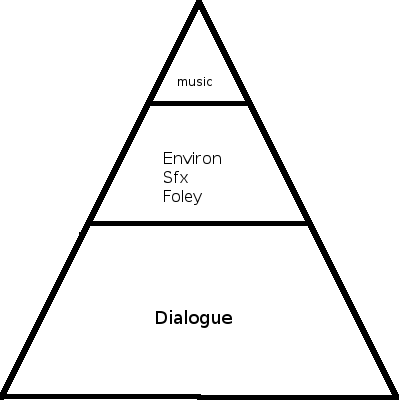
\includegraphics[scale=2.0]{triangleoffilm} 

\subsection{Simple examples}
\begin{itemize}
\item Melodic writing
\item eg. Married life video from `Up' (a waltz in the original)
\item Manuscript paper hand-out and write 16 bars. I then played them back on the violin
\item Star Wars (Throne room scene: A march)
\item Examples: John Carter (2012, Stanton, music - Giacchino)
\end{itemize}

\subsection{Bring me sunshine} 
\begin{itemize}
\item Play clip from the film Sunshine (Danny Boyle - 2007) 
\item Spot a piece of music from Naxos of your choice to it
\item Brahms1 score copy from handout in Sibelius and MuseScore 
\item Add video
\item Introducing spotting music to clips and familiarity with Sibelius and/or MuseScore
\end{itemize}


\subsection{More spotting}
\begin{itemize}
\item Gladiator (Title 1, chapter 2 - battle scene)
\item spot with Mars (Holst) / compare original
\item Compose to the `battle' clip (see wiki) - piano only
\end{itemize}

\section{Orchestration}
\begin{itemize}
\item As the wiki - winds (Stravinsky), brass (Janacek, Copland): Copy and alter in MuseScore
\item Spot film clip to music
\item Examples. Vertigo (1958, Hitchcock - Hermann); Scott of the Antarctic (1948, Vaughan Williams); 
\item Robin Hood 1938, Korngold score; 1991, Dir: Kevin Reynolds, Music - Michael Kamen; 2010, Dir. Ridley Scott, Music - Marc Streitenfeld  
\end{itemize}

\section{Sfx}
\begin{itemize}
\item Examples: Bourne sfx; Wall-e; THX1138

\end{itemize}

\section{Writing something more experimental}
\begin{itemize}
\item This assignment involves the use of Cubase and a more sfx / electroacoustic piece
\item The film choice should therefore be potentially `atmospheric'
\item Students can be introduced to the USSStoolkit and granulate some simple sounds
\item Students may wish to borrow portable recorders to make their own sfx/foley
\item \textit{We don't do a session on foley, mainly because we don't have the facilities. It might be fun in the future}
\item This assignment can also be a popular music track - it just can't be another WCM example. 
\item Examples: Clockwork Orange (1971, Wendy Carlos); Bladerunner (1982, Vangelis); Social Network (2010, Trent Reznor, Atticus Ross); Forbidden Planet (1956, Barron); The Birds (1963, Hitchcock, Sala and the Trautonium)
\end{itemize}

\section{Visual Music}
\begin{itemize}
\item Examples of AV pieces where (in many cases) the composer is also the video artist. 
\item Introduce students to Processing and Blender - just to say that they are out there. 
\item Have a look at GEM in puredata 
\item Examples: Brett Battey; Louise Harris
\end{itemize}

\section{Taking MUS340 forward}
\begin{itemize}
\item I would really like them to score for the instruments in the class then conduct to picture. Tricky to organise
\item I mainly expect them to provide the clip of the original film and the clip with their music
\item Q: `but if I rip the film, I lose the dialogue and sfx,. Will I lose marks for not putting them back in'. A: No, but why would you not want to make your clip as perfect as possible. Those that have in the past were the ones that felt most proud about their work and got the most out of the course
\item Q: `can I rip my favourite film?' A: Yes, but it will potentially be useless to score to. Hollywood isn't great for finding something really creative to work with. Try also to find a finished `short'. Some films will not be around five minutes (plus/minus). Obviously there are times when students want to `get away with it'. This is always obvious in the final submission. 
\end{itemize}

\section{Opportunities: really important}
\begin{itemize}
\item South Yorkshire Filmmakers Network \url{http://syfn.org/}
\item If considering taking an special project module or extended special project with film music scoring as an outcome, scoring to materials downloaded from the internet is not allowed. You MUST find a film maker and document your process. Therefore, syfn is the place to get involved. 
\end{itemize}

\section{Student work}
\begin{itemize}
\item Play past examples and pick apart
\end{itemize}



